% ================================================================
% Chapter 2 � Space and Time Domain (DOM)
% ================================================================
\chapter{Space Domain (DOM) }
\label{DOM}
\minitoc

% Missing things:
% 	- istate: description of the initial state   ==> this has to be put elsewhere..
%                  perhaps in MISC ?  By the way the initialisation of T S and dynamics 
%                  should be put outside of DOM routine (better with TRC staff and off-line
%                  tracers)
% 	-geo2ocean:  how to switch from geographic to mesh coordinate
%     - domclo:  closed sea and lakes.... management of closea sea area : specific to global configuration, both forced and coupled


\newpage
$\ $\newline    % force a new ligne

Having defined the continuous equations in Chap.~\ref{PE} and chosen a time 
discretization Chap.~\ref{STP}, we need to choose a discretization on a grid, 
and numerical algorithms. In the present chapter, we provide a general description 
of the staggered grid used in \NEMO, and other information relevant to the main 
directory routines as well as the DOM (DOMain) directory. 

$\ $\newline    % force a new lign

% ================================================================
% Fundamentals of the Discretisation
% ================================================================
\section{Fundamentals of the Discretisation}
\label{DOM_basics}

% -------------------------------------------------------------------------------------------------------------
%        Arrangement of Variables 
% -------------------------------------------------------------------------------------------------------------
\subsection{Arrangement of Variables}
\label{DOM_cell}

%>>>>>>>>>>>>>>>>>>>>>>>>>>>>
\begin{figure}[!tb]    \begin{center}
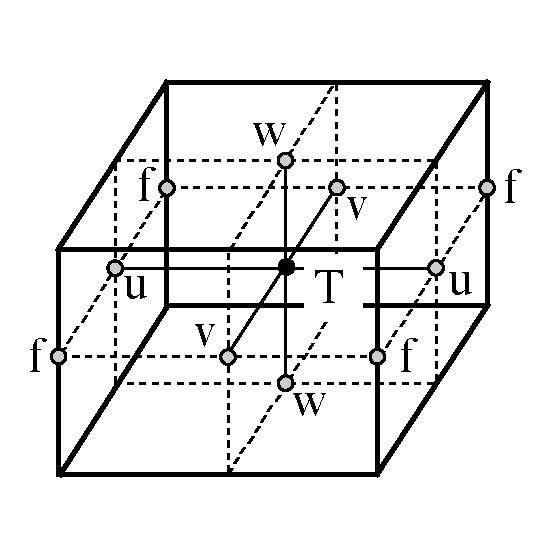
\includegraphics[width=0.90\textwidth]{./TexFiles/Figures/Fig_cell.pdf}
\caption{ \label{Fig_cell}    
Arrangement of variables. $t$ indicates scalar points where temperature, 
salinity, density, pressure and horizontal divergence are defined. ($u$,$v$,$w$) 
indicates vector points, and $f$ indicates vorticity points where both relative and 
planetary vorticities are defined}
\end{center}   \end{figure}
%>>>>>>>>>>>>>>>>>>>>>>>>>>>>

The numerical techniques used to solve the Primitive Equations in this model are 
based on the traditional, centred second-order finite difference approximation. 
Special attention has been given to the homogeneity of the solution in the three 
space directions. The arrangement of variables is the same in all directions. 
It consists of cells centred on scalar points ($t$, $S$, $p$, $\rho$) with vector 
points $(u, v, w)$ defined in the centre of each face of the cells (Fig. \ref{Fig_cell}). 
This is the generalisation to three dimensions of the well-known ``C'' grid in 
Arakawa's classification \citep{Mesinger_Arakawa_Bk76}. The relative and 
planetary vorticity, $\zeta$ and $f$, are defined in the centre of each vertical edge 
and the barotropic stream function $\psi$ is defined at horizontal points overlying 
the $\zeta$ and $f$-points.

The ocean mesh ($i.e.$ the position of all the scalar and vector points) is defined 
by the transformation that gives ($\lambda$ ,$\varphi$ ,$z$) as a function of $(i,j,k)$. 
The grid-points are located at integer or integer and a half value of $(i,j,k)$ as 
indicated on Table \ref{Tab_cell}. In all the following, subscripts $u$, $v$, $w$, 
$f$, $uw$, $vw$ or $fw$ indicate the position of the grid-point where the scale 
factors are defined. Each scale factor is defined as the local analytical value 
provided by \eqref{Eq_scale_factors}. As a result, the mesh on which partial 
derivatives $\frac{\partial}{\partial \lambda}, \frac{\partial}{\partial \varphi}$, and 
$\frac{\partial}{\partial z} $ are evaluated is a uniform mesh with a grid size of unity. 
Discrete partial derivatives are formulated by the traditional, centred second order 
finite difference approximation while the scale factors are chosen equal to their 
local analytical value. An important point here is that the partial derivative of the 
scale factors must be evaluated by centred finite difference approximation, not 
from their analytical expression. This preserves the symmetry of the discrete set 
of equations and therefore satisfies many of the continuous properties (see 
Appendix~\ref{Apdx_C}). A similar, related remark can be made about the domain 
size: when needed, an area, volume, or the total ocean depth must be evaluated 
as the sum of the relevant scale factors (see \eqref{DOM_bar}) in the next section). 

%>>>>>>>>>>>>>>>>>>>>>>>>>>>>
\begin{table}[!tb]
\begin{center} \begin{tabular}{|p{46pt}|p{56pt}|p{56pt}|p{56pt}|}
\hline
T	&$i$ 		& $j$		& $k$		 \\ \hline
u	& $i+1/2$	& $j$		& $k$	 	\\ \hline
v	& $i$	 	& $j+1/2$	& $k$	 	\\ \hline
w	& $i$	 	& $j$		& $k+1/2$ 	\\ \hline
f	& $i+1/2$ 	& $j+1/2$	& $k$	 	\\ \hline
uw	& $i+1/2$ 	& $j$		& $k+1/2$ 	\\ \hline
vw	& $i$	 	& $j+1/2$	& $k+1/2$ 	\\ \hline
fw	& $i+1/2$ 	& $j+1/2$	& $k+1/2$ 	\\ \hline
\end{tabular}
\caption{ \label{Tab_cell}
Location of grid-points as a function of integer or integer and a half value of the column, 
line or level. This indexing is only used for the writing of the semi-discrete equation. 
In the code, the indexing uses integer values only and has a reverse direction 
in the vertical (see \S\ref{DOM_Num_Index})}
\end{center}
\end{table}
%>>>>>>>>>>>>>>>>>>>>>>>>>>>>

% -------------------------------------------------------------------------------------------------------------
%        Vector Invariant Formulation 
% -------------------------------------------------------------------------------------------------------------
\subsection{Discrete Operators}
\label{DOM_operators}

Given the values of a variable $q$ at adjacent points, the differencing and 
averaging operators at the midpoint between them are:
\begin{subequations} \label{Eq_di_mi}
\begin{align}
 \delta _i [q]       &=  \  \    q(i+1/2)  - q(i-1/2)		\\
 \overline q^{\,i} &= \left\{ q(i+1/2) + q(i-1/2) \right\} \; / \; 2
\end{align}
\end{subequations}

Similar operators are defined with respect to $i+1/2$, $j$, $j+1/2$, $k$, and 
$k+1/2$. Following \eqref{Eq_PE_grad} and \eqref{Eq_PE_lap}, the gradient of a 
variable $q$ defined at a $t$-point has its three components defined at $u$-, $v$- 
and $w$-points while its Laplacien is defined at $t$-point. These operators have 
the following discrete forms in the curvilinear $s$-coordinate system:
\begin{equation} \label{Eq_DOM_grad}
\nabla q\equiv 	\frac{1}{e_{1u} } \delta _{i+1/2 } [q] \;\,\mathbf{i}
		+	\frac{1}{e_{2v} } \delta _{j+1/2 } [q] \;\,\mathbf{j}
		+	\frac{1}{e_{3w}} \delta _{k+1/2} [q] \;\,\mathbf{k}
\end{equation}
\begin{multline} \label{Eq_DOM_lap}
\Delta q\equiv \frac{1}{e_{1t}\,e_{2t}\,e_{3t} }
       \;\left(          \delta_i  \left[ \frac{e_{2u}\,e_{3u}} {e_{1u}} \;\delta_{i+1/2} [q] \right]
+                        \delta_j  \left[ \frac{e_{1v}\,e_{3v}}  {e_{2v}} \;\delta_{j+1/2} [q] \right] \;  \right)		\\
+\frac{1}{e_{3t}} \delta_k \left[ \frac{1}{e_{3w} }                     \;\delta_{k+1/2} [q] \right]
\end{multline}

Following \eqref{Eq_PE_curl} and \eqref{Eq_PE_div}, a vector ${\rm {\bf A}}=\left( a_1,a_2,a_3\right)$ 
defined at vector points $(u,v,w)$ has its three curl components defined at $vw$-, $uw$, 
and $f$-points, and its divergence defined at $t$-points:
\begin{eqnarray}  \label{Eq_DOM_curl}
 \nabla \times {\rm {\bf A}}\equiv &
      \frac{1}{e_{2v}\,e_{3vw} } \ \left( \delta_{j +1/2} \left[e_{3w}\,a_3 \right] -\delta_{k+1/2} \left[e_{2v} \,a_2 \right] \right)  &\ \mathbf{i} \\ 
 +& \frac{1}{e_{2u}\,e_{3uw}} \ \left( \delta_{k+1/2} \left[e_{1u}\,a_1  \right] -\delta_{i +1/2} \left[e_{3w}\,a_3 \right] \right)  &\ \mathbf{j} \\
 +& \frac{1}{e_{1f} \,e_{2f}    } \ \left( \delta_{i +1/2} \left[e_{2v}\,a_2  \right] -\delta_{j +1/2} \left[e_{1u}\,a_1 \right] \right)  &\ \mathbf{k}
 \end{eqnarray}
\begin{equation} \label{Eq_DOM_div}
\nabla \cdot \rm{\bf A}=\frac{1}{e_{1t}\,e_{2t}\,e_{3t}}\left( \delta_i \left[e_{2u}\,e_{3u}\,a_1 \right]
                                                                                         +\delta_j \left[e_{1v}\,e_{3v}\,a_2 \right] \right)+\frac{1}{e_{3t} }\delta_k \left[a_3 \right]
\end{equation}

In the special case of a pure $z$-coordinate system, \eqref{Eq_DOM_lap} and 
\eqref{Eq_DOM_div} can be simplified. In this case, the vertical scale factor 
becomes a function of the single variable $k$ and thus does not depend on the 
horizontal location of a grid point. For example \eqref{Eq_DOM_div} reduces to: 
\begin{equation*}
\nabla \cdot \rm{\bf A}=\frac{1}{e_{1t}\,e_{2t}} \left( \delta_i \left[e_{2u}\,a_1 \right] 
                                                                              +\delta_j \left[e_{1v}\, a_2 \right]  \right)
                                                     +\frac{1}{e_{3t}} \delta_k \left[             a_3 \right]
\end{equation*}

The vertical average over the whole water column denoted by an overbar becomes 
for a quantity $q$ which is a masked field (i.e. equal to zero inside solid area):
\begin{equation} \label{DOM_bar}
\bar q 	=         \frac{1}{H}    \int_{k^b}^{k^o} {q\;e_{3q} \,dk} 
		\equiv \frac{1}{H_q }\sum\limits_k {q\;e_{3q} }
\end{equation}
where $H_q$  is the ocean depth, which is the masked sum of the vertical scale 
factors at $q$ points, $k^b$ and $k^o$ are the bottom and surface $k$-indices, 
and the symbol $k^o$ refers to a summation over all grid points of the same type 
in the direction indicated by the subscript (here $k$). 

In continuous form, the following properties are satisfied:
\begin{equation} \label{Eq_DOM_curl_grad}
\nabla \times \nabla q ={\rm {\bf {0}}}
\end{equation}
\begin{equation} \label{Eq_DOM_div_curl}
\nabla \cdot \left( {\nabla \times {\rm {\bf A}}} \right)=0
\end{equation}

It is straightforward to demonstrate that these properties are verified locally in 
discrete form as soon as the scalar $q$ is taken at $t$-points and the vector 
\textbf{A} has its components defined at vector points $(u,v,w)$.

Let $a$ and $b$ be two fields defined on the mesh, with value zero inside 
continental area. Using integration by parts it can be shown that the differencing 
operators ($\delta_i$, $\delta_j$ and $\delta_k$) are anti-symmetric linear 
operators, and further that the averaging operators $\overline{\,\cdot\,}^{\,i}$, 
$\overline{\,\cdot\,}^{\,k}$ and $\overline{\,\cdot\,}^{\,k}$) are symmetric linear 
operators, $i.e.$
\begin{align} 
\label{DOM_di_adj}
\sum\limits_i { a_i \;\delta _i \left[ b \right]} 
	&\equiv -\sum\limits_i {\delta _{i+1/2} \left[ a \right]\;b_{i+1/2} }      \\
\label{DOM_mi_adj}
\sum\limits_i { a_i \;\overline b^{\,i}} 
	& \equiv \quad \sum\limits_i {\overline a ^{\,i+1/2}\;b_{i+1/2} } 
\end{align}

In other words, the adjoint of the differencing and averaging operators are 
$\delta_i^*=\delta_{i+1/2}$ and 
${(\overline{\,\cdot \,}^{\,i})}^*= \overline{\,\cdot\,}^{\,i+1/2}$, respectively. 
These two properties will be used extensively in the Appendix~\ref{Apdx_C} to 
demonstrate integral conservative properties of the discrete formulation chosen.

% -------------------------------------------------------------------------------------------------------------
%        Numerical Indexing 
% -------------------------------------------------------------------------------------------------------------
\subsection{Numerical Indexing}
\label{DOM_Num_Index}

%>>>>>>>>>>>>>>>>>>>>>>>>>>>>
\begin{figure}[!tb]  \begin{center}
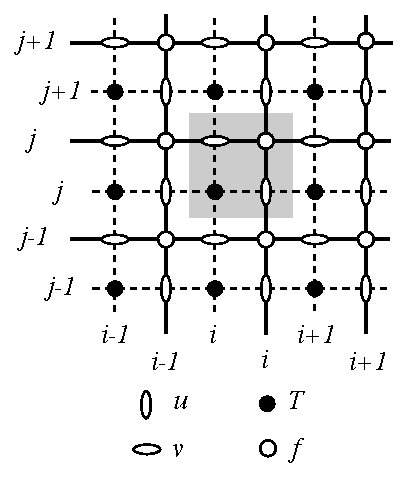
\includegraphics[width=0.90\textwidth]{./TexFiles/Figures/Fig_index_hor.pdf}
\caption{   \label{Fig_index_hor}    
Horizontal integer indexing used in the \textsc{Fortran} code. The dashed area indicates 
the cell in which variables contained in arrays have the same $i$- and $j$-indices}
\end{center}   \end{figure}
%>>>>>>>>>>>>>>>>>>>>>>>>>>>>

The array representation used in the \textsc{Fortran} code requires an integer 
indexing while the analytical definition of the mesh (see \S\ref{DOM_cell}) is 
associated with the use of integer values for $t$-points and both integer and 
integer and a half values for all the other points. Therefore a specific integer 
indexing must be defined for points other than $t$-points ($i.e.$ velocity and 
vorticity grid-points). Furthermore, the direction of the vertical indexing has 
been changed so that the surface level is at $k=1$.

% -----------------------------------
%        Horizontal Indexing 
% -----------------------------------
\subsubsection{Horizontal Indexing}
\label{DOM_Num_Index_hor}

The indexing in the horizontal plane has been chosen as shown in Fig.\ref{Fig_index_hor}. 
For an increasing $i$ index ($j$ index), the $t$-point and the eastward $u$-point 
(northward $v$-point) have the same index (see the dashed area in Fig.\ref{Fig_index_hor}). 
A $t$-point and its nearest northeast $f$-point have the same $i$-and $j$-indices.

% -----------------------------------
%        Vertical indexing 
% -----------------------------------
\subsubsection{Vertical Indexing}
\label{DOM_Num_Index_vertical}

In the vertical, the chosen indexing requires special attention since the 
$k$-axis is re-orientated downward in the \textsc{Fortran} code compared 
to the indexing used in the semi-discrete equations and given in \S\ref{DOM_cell}. 
The sea surface corresponds to the $w$-level $k=1$ which is the same index 
as $t$-level just below (Fig.\ref{Fig_index_vert}). The last $w$-level ($k=jpk$) 
either corresponds to the ocean floor or is inside the bathymetry while the last 
$t$-level is always inside the bathymetry (Fig.\ref{Fig_index_vert}). Note that 
for an increasing $k$ index, a $w$-point and the $t$-point just below have the 
same $k$ index, in opposition to what is done in the horizontal plane where 
it is the $t$-point and the nearest velocity points in the direction of the horizontal 
axis that have the same $i$ or $j$ index (compare the dashed area in 
Fig.\ref{Fig_index_hor} and \ref{Fig_index_vert}). Since the scale factors are 
chosen to be strictly positive, a \emph{minus sign} appears in the \textsc{Fortran} 
code \emph{before all the vertical derivatives} of the discrete equations given in 
this documentation.

%>>>>>>>>>>>>>>>>>>>>>>>>>>>>
\begin{figure}[!pt]    \begin{center}
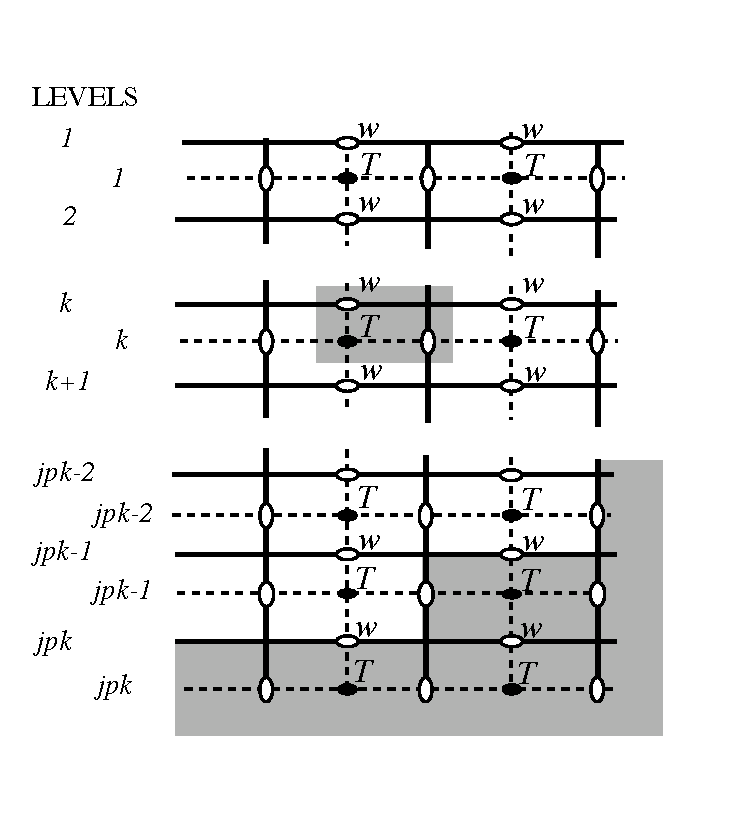
\includegraphics[width=.90\textwidth]{./TexFiles/Figures/Fig_index_vert.pdf}
\caption{ \label{Fig_index_vert}     
Vertical integer indexing used in the \textsc{Fortran } code. Note that 
the $k$-axis is orientated downward. The dashed area indicates the cell in 
which variables contained in arrays have the same $k$-index.}
\end{center}   \end{figure}
%>>>>>>>>>>>>>>>>>>>>>>>>>>>>

% -----------------------------------
%        Domain Size
% -----------------------------------
\subsubsection{Domain Size}
\label{DOM_size}

The total size of the computational domain is set by the parameters \np{jpiglo}, 
\np{jpjglo} and \np{jpkdta} in the $i$, $j$ and $k$ directions respectively. They are 
given as namelist variables in the \ngn{namcfg} namelist. 

Note that are other namelist variables in the \ngn{namcfg} namelist that refer to
 the domain size. 
The two variables \np{jpidta} and \np{jpjdta} may be larger than \np{jpiglo}, \np{jpjglo}
when the user wants to use only a sub-region of a given configuration. This is 
the "zoom" capability described in \S\ref{MISC_zoom}. In most applications of 
the model, $jpidta=jpiglo$, $jpjdta=jpjglo$, and $jpizoom=jpjzoom=1$. Parameters 
$jpi$ and $jpj$ refer to the size of each processor subdomain when the code is 
run in parallel using domain decomposition (\key{mpp\_mpi} defined, see 
\S\ref{LBC_mpp}).


$\ $\newline    % force a new lign

% ================================================================
% Domain: Horizontal Grid (mesh) 
% ================================================================
\section  [Domain: Horizontal Grid (mesh) (\textit{domhgr})]               
		{Domain: Horizontal Grid (mesh) \small{(\mdl{domhgr} module)} }
\label{DOM_hgr}

% -------------------------------------------------------------------------------------------------------------
%        Coordinates and scale factors 
% -------------------------------------------------------------------------------------------------------------
\subsection{Coordinates and scale factors}
\label{DOM_hgr_coord_e}

The ocean mesh ($i.e.$ the position of all the scalar and vector points) is defined 
by the transformation that gives $(\lambda,\varphi,z)$ as a function of $(i,j,k)$. 
The grid-points are located at integer or integer and a half values of as indicated 
in Table~\ref{Tab_cell}. The associated scale factors are defined using the 
analytical first derivative of the transformation \eqref{Eq_scale_factors}. These 
definitions are done in two modules, \mdl{domhgr} and \mdl{domzgr}, which 
provide the horizontal and vertical meshes, respectively. This section deals with 
the horizontal mesh parameters.

In a horizontal plane, the location of all the model grid points is defined from the 
analytical expressions of the longitude $\lambda$ and  latitude $\varphi$ as a 
function of  $(i,j)$. The horizontal scale factors are calculated using 
\eqref{Eq_scale_factors}. For example, when the longitude and latitude are 
function of a single value ($i$ and $j$, respectively) (geographical configuration 
of the mesh), the horizontal mesh definition reduces to define the wanted 
$\lambda(i)$, $\varphi(j)$, and their derivatives $\lambda'(i)$ $\varphi'(j)$ in the 
\mdl{domhgr} module. The model computes the grid-point positions and scale 
factors in the horizontal plane as follows:
\begin{flalign*}
\lambda_t &\equiv \text{glamt}= \lambda(i)	  & \varphi_t &\equiv \text{gphit} = \varphi(j)\\
\lambda_u &\equiv \text{glamu}= \lambda(i+1/2)& \varphi_u &\equiv \text{gphiu}= \varphi(j)\\
\lambda_v &\equiv \text{glamv}= \lambda(i)       & \varphi_v &\equiv \text{gphiv} = \varphi(j+1/2)\\
\lambda_f &\equiv \text{glamf }= \lambda(i+1/2)& \varphi_f &\equiv \text{gphif }= \varphi(j+1/2) 
\end{flalign*}
\begin{flalign*}
e_{1t} &\equiv \text{e1t} = r_a |\lambda'(i)		\; \cos\varphi(j)  |&
e_{2t} &\equiv \text{e2t} = r_a |\varphi'(j)|  \\
e_{1u} &\equiv \text{e1t} = r_a |\lambda'(i+1/2)	\; \cos\varphi(j)  |&
e_{2u} &\equiv \text{e2t} = r_a |\varphi'(j)|\\
e_{1v} &\equiv \text{e1t} = r_a |\lambda'(i)		\; \cos\varphi(j+1/2)  |&
e_{2v} &\equiv \text{e2t} = r_a |\varphi'(j+1/2)|\\
e_{1f} &\equiv \text{e1t} = r_a |\lambda'(i+1/2)\; \cos\varphi(j+1/2)  |&
e_{2f} &\equiv \text{e2t} = r_a |\varphi'(j+1/2)|
\end{flalign*}
where the last letter of each computational name indicates the grid point 
considered and $r_a$ is the earth radius (defined in \mdl{phycst} along with 
all universal constants). Note that the horizontal position of and scale factors 
at $w$-points are exactly equal to those of $t$-points, thus no specific arrays 
are defined at $w$-points. 

Note that the definition of the scale factors ($i.e.$ as the analytical first derivative 
of the transformation that gives $(\lambda,\varphi,z)$ as a function of $(i,j,k)$) is 
specific to the \NEMO model \citep{Marti_al_JGR92}. As an example, $e_{1t}$ is defined 
locally at a $t$-point, whereas many other models on a C grid choose to define 
such a scale factor as the distance between the $U$-points on each side of the 
$t$-point. Relying on an analytical transformation has two advantages: firstly, there 
is no ambiguity in the scale factors appearing in the discrete equations, since they 
are first introduced in the continuous equations; secondly, analytical transformations 
encourage good practice by the definition of smoothly varying grids (rather than 
allowing the user to set arbitrary jumps in thickness between adjacent layers) 
\citep{Treguier1996}. An example of the effect of such a choice is shown in 
Fig.~\ref{Fig_zgr_e3}.
%>>>>>>>>>>>>>>>>>>>>>>>>>>>>
\begin{figure}[!t]     \begin{center}
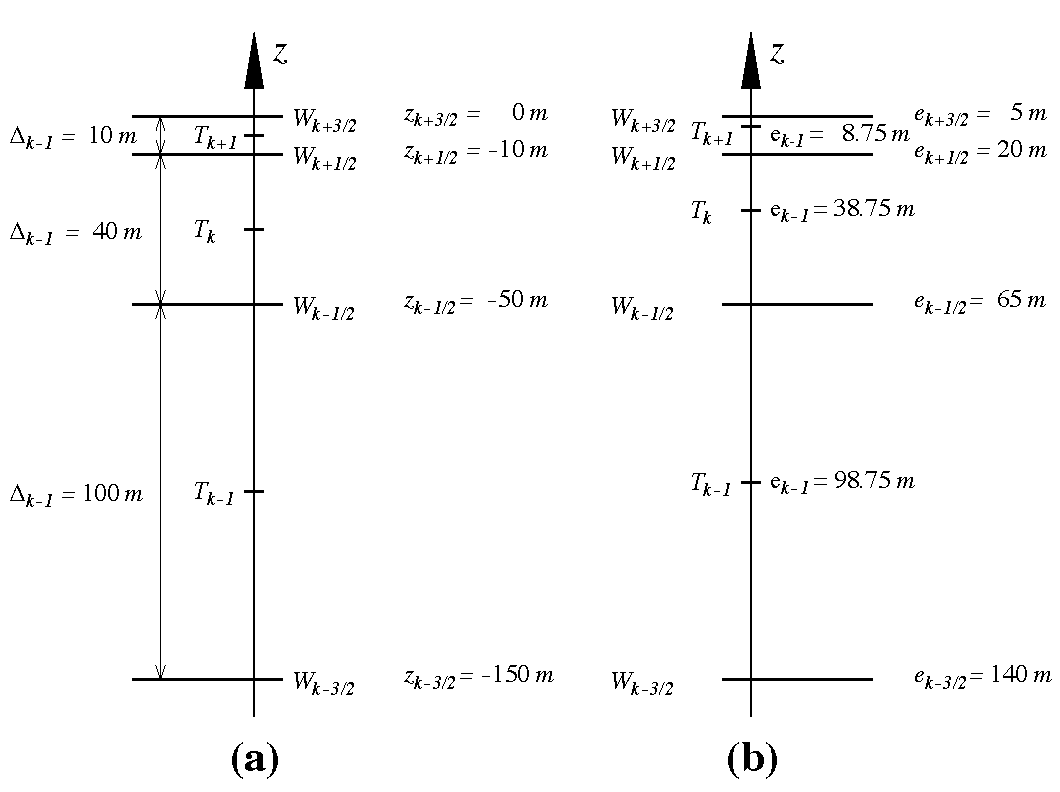
\includegraphics[width=0.90\textwidth]{./TexFiles/Figures/Fig_zgr_e3.pdf}
\caption{ \label{Fig_zgr_e3}    
Comparison of (a) traditional definitions of grid-point position and grid-size in the vertical, 
and (b) analytically derived grid-point position and scale factors. 
For both grids here,  the same $w$-point depth has been chosen but in (a) the 
$t$-points are set half way between $w$-points while in (b) they are defined from 
an analytical function: $z(k)=5\,(i-1/2)^3 - 45\,(i-1/2)^2 + 140\,(i-1/2) - 150$. 
Note the resulting difference between the value of the grid-size $\Delta_k$ and 
those of the scale factor $e_k$. }
\end{center}   \end{figure}
%>>>>>>>>>>>>>>>>>>>>>>>>>>>>

% -------------------------------------------------------------------------------------------------------------
%        Choice of horizontal grid
% -------------------------------------------------------------------------------------------------------------
\subsection{Choice of horizontal grid}
\label{DOM_hgr_msh_choice}

The user has three options available in defining a horizontal grid, which involve 
the namelist variable \np{jphgr\_mesh} of the \ngn{namcfg} namelist. 
\begin{description}
\item[\np{jphgr\_mesh}=0]  The most general curvilinear orthogonal grids.
The coordinates and their first derivatives with respect to $i$ and $j$ are provided
in a input file (\ifile{coordinates}), read in \rou{hgr\_read} subroutine of the domhgr module.
\item[\np{jphgr\_mesh}=1 to 5] A few simple analytical grids are provided (see below). 
For other analytical grids, the \mdl{domhgr} module must be modified by the user. 
\end{description}

There are two simple cases of geographical grids on the sphere. With 
\np{jphgr\_mesh}=1, the grid (expressed in degrees) is regular in space, 
with grid sizes specified by parameters \np{ppe1\_deg} and \np{ppe2\_deg}, 
respectively. Such a geographical grid can be very anisotropic at high latitudes 
because of the convergence of meridians (the zonal scale factors $e_1$ 
become much smaller than the meridional scale factors $e_2$). The Mercator 
grid (\np{jphgr\_mesh}=4) avoids this anisotropy by refining the meridional scale 
factors in the same way as the zonal ones. In this case, meridional scale factors 
and latitudes are calculated analytically using the formulae appropriate for 
a Mercator projection, based on \np{ppe1\_deg} which is a reference grid spacing 
at the equator (this applies even when the geographical equator is situated outside 
the model domain). 
%%%
\gmcomment{ give here the analytical expression of the Mercator mesh}
%%%
In these two cases (\np{jphgr\_mesh}=1 or 4), the grid position is defined by the 
longitude and latitude of the south-westernmost point (\np{ppglamt0} 
and \np{ppgphi0}). Note that for the Mercator grid the user need only provide 
an approximate starting latitude: the real latitude will be recalculated analytically, 
in order to ensure that the equator corresponds to line passing through $t$- 
and $u$-points.  

Rectangular grids ignoring the spherical geometry are defined with 
\np{jphgr\_mesh} = 2, 3, 5. The domain is either an $f$-plane (\np{jphgr\_mesh} = 2, 
Coriolis factor is constant) or a beta-plane (\np{jphgr\_mesh} = 3, the Coriolis factor 
is linear in the $j$-direction). The grid size is uniform in meter in each direction, 
and given by the parameters \np{ppe1\_m} and \np{ppe2\_m} respectively. 
The zonal grid coordinate (\textit{glam} arrays) is in kilometers, starting at zero 
with the first $t$-point. The meridional coordinate (gphi. arrays) is in kilometers, 
and the second $t$-point corresponds to coordinate $gphit=0$. The input 
variable \np{ppglam0} is ignored. \np{ppgphi0} is used to set the reference 
latitude for computation of the Coriolis parameter. In the case of the beta plane, 
\np{ppgphi0} corresponds to the center of the domain. Finally, the special case 
\np{jphgr\_mesh}=5 corresponds to a beta plane in a rotated domain for the 
GYRE configuration, representing a classical mid-latitude double gyre system. 
The rotation allows us to maximize the jet length relative to the gyre areas 
(and the number of grid points). 

The choice of the grid must be consistent with the boundary conditions specified 
by the parameter \np{jperio} (see {\S\ref{LBC}).

% -------------------------------------------------------------------------------------------------------------
%        Grid files
% -------------------------------------------------------------------------------------------------------------
\subsection{Output Grid files}
\label{DOM_hgr_files}

All the arrays relating to a particular ocean model configuration (grid-point 
position, scale factors, masks) can be saved in files if $\np{nn\_msh} \not= 0$ 
(namelist variable in \ngn{namdom}). This can be particularly useful for plots and off-line 
diagnostics. In some cases, the user may choose to make a local modification 
of a scale factor in the code. This is the case in global configurations when 
restricting the width of a specific strait (usually a one-grid-point strait that 
happens to be too wide due to insufficient model resolution). An example 
is Gibraltar Strait in the ORCA2 configuration. When such modifications are done, 
the output grid written when $\np{nn\_msh} \not=0$ is no more equal to the input grid.

$\ $\newline    % force a new lign

% ================================================================
% Domain: Vertical Grid (domzgr)
% ================================================================
\section  [Domain: Vertical Grid (\textit{domzgr})]
		{Domain: Vertical Grid \small{(\mdl{domzgr} module)} }
\label{DOM_zgr}
%-----------------------------------------nam_zgr & namdom-------------------------------------------
\namdisplay{namzgr} 
\namdisplay{namdom} 
%-------------------------------------------------------------------------------------------------------------

Variables are defined through the \ngn{namzgr} and \ngn{namdom} namelists.
In the vertical, the model mesh is determined by four things: 
(1) the bathymetry given in meters ; 
(2) the number of levels of the model (\jp{jpk}) ; 
(3) the analytical transformation $z(i,j,k)$ and the vertical scale factors 
(derivatives of the transformation) ; 
and (4) the masking system, $i.e.$ the number of wet model levels at each 
$(i,j)$ column of points.

%>>>>>>>>>>>>>>>>>>>>>>>>>>>>
\begin{figure}[!tb]    \begin{center}
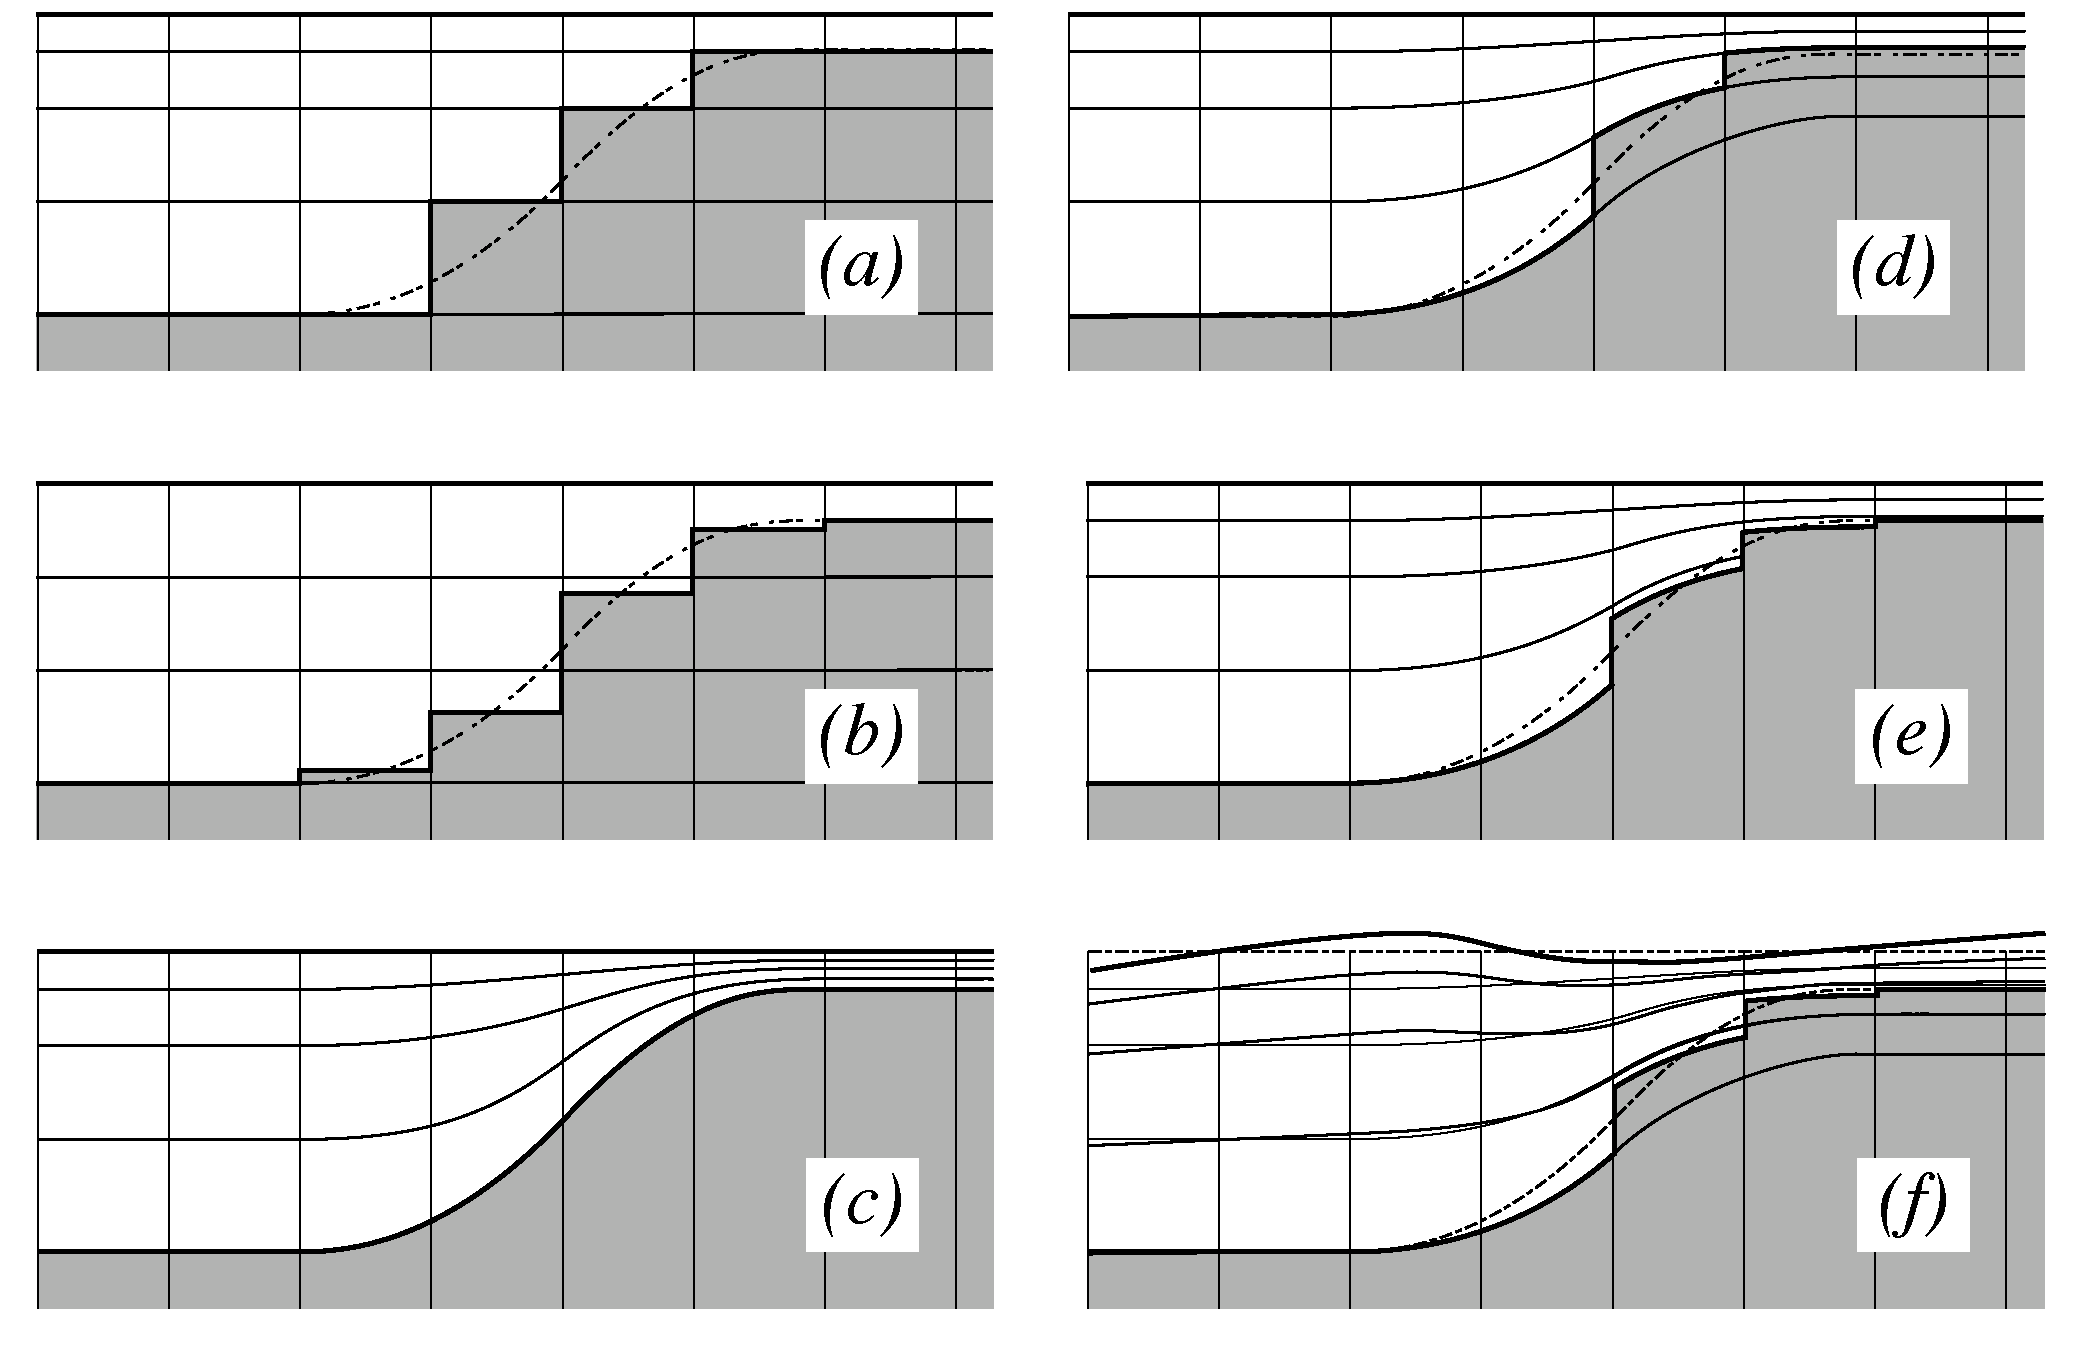
\includegraphics[width=1.0\textwidth]{./TexFiles/Figures/Fig_z_zps_s_sps.pdf}
\caption{  \label{Fig_z_zps_s_sps}   
The ocean bottom as seen by the model: 
(a) $z$-coordinate with full step, 
(b) $z$-coordinate with partial step, 
(c) $s$-coordinate: terrain following representation, 
(d) hybrid $s-z$ coordinate, 
(e) hybrid $s-z$ coordinate with partial step, and 
(f) same as (e) but with variable volume associated with the non-linear free surface. 
Note that the variable volume option (\key{vvl}) can be used with any of the 
5 coordinates (a) to (e).}
\end{center}   \end{figure}
%>>>>>>>>>>>>>>>>>>>>>>>>>>>>

The choice of a vertical coordinate, even if it is made through a namelist parameter, 
must be done once of all at the beginning of an experiment. It is not intended as an 
option which can be enabled or disabled in the middle of an experiment. Three main 
choices are offered (Fig.~\ref{Fig_z_zps_s_sps}a to c): $z$-coordinate with full step 
bathymetry (\np{ln\_zco}~=~true), $z$-coordinate with partial step bathymetry 
(\np{ln\_zps}~=~true), or generalized, $s$-coordinate (\np{ln\_sco}~=~true). 
Hybridation of the three main coordinates are available: $s-z$ or $s-zps$ coordinate 
(Fig.~\ref{Fig_z_zps_s_sps}d and \ref{Fig_z_zps_s_sps}e). When using the variable 
volume option \key{vvl} ($i.e.$ non-linear free surface), the coordinate follow the 
time-variation of the free surface so that the transformation is time dependent: 
$z(i,j,k,t)$ (Fig.~\ref{Fig_z_zps_s_sps}f). This option can be used with full step 
bathymetry or $s$-coordinate (hybrid and partial step coordinates have not 
yet been tested in NEMO v2.3). If using $z$-coordinate with partial step bathymetry
(\np{ln\_zps}~=~true), ocean cavity beneath ice shelves can be open (\np{ln\_isfcav}~=~true).

Contrary to the horizontal grid, the vertical grid is computed in the code and no 
provision is made for reading it from a file. The only input file is the bathymetry 
(in meters) (\ifile{bathy\_meter}) 
\footnote{N.B. in full step $z$-coordinate, a \ifile{bathy\_level} file can replace the 
\ifile{bathy\_meter} file, so that the computation of the number of wet ocean point 
in each water column is by-passed}. 
After reading the bathymetry, the algorithm for vertical grid definition differs 
between the different options:
\begin{description}
\item[\textit{zco}] set a reference coordinate transformation $z_0 (k)$, and set $z(i,j,k,t)=z_0 (k)$.
\item[\textit{zps}] set a reference coordinate transformation $z_0 (k)$, and 
calculate the thickness of the deepest level at each $(i,j)$ point using the 
bathymetry, to obtain the final three-dimensional depth and scale factor arrays.
\item[\textit{sco}] smooth the bathymetry to fulfil the hydrostatic consistency 
criteria and set the three-dimensional transformation.
\item[\textit{s-z} and \textit{s-zps}] smooth the bathymetry to fulfil the hydrostatic 
consistency criteria and set the three-dimensional transformation $z(i,j,k)$, and 
possibly introduce masking of extra land points to better fit the original bathymetry file
\end{description}
%%%
\gmcomment{   add the description of the smoothing:  envelop topography...}
%%%

The arrays describing the grid point depths and vertical scale factors 
are three dimensional arrays $(i,j,k)$ even in the case of $z$-coordinate with 
full step bottom topography. In non-linear free surface (\key{vvl}), their knowledge
is required at \textit{before}, \textit{now} and \textit{after} time step, while they 
do not vary in time in linear free surface case. 
To improve the code readability while providing this flexibility, the vertical coordinate 
and scale factors are defined as functions of 
$(i,j,k)$ with "fs" as prefix (examples: \textit{fse3t\_b, fse3t\_n, fse3t\_a,} 
for the  \textit{before}, \textit{now} and \textit{after} scale factors at $t$-point) 
that can be either three different arrays when \key{vvl} is defined, or a single fixed arrays. 
These functions are defined in the file \hf{domzgr\_substitute} of the DOM directory. 
They are used throughout the code, and replaced by the corresponding arrays at 
the time of pre-processing (CPP capability).

% -------------------------------------------------------------------------------------------------------------
%        Meter Bathymetry
% -------------------------------------------------------------------------------------------------------------
\subsection{Meter Bathymetry}
\label{DOM_bathy}

Three options are possible for defining the bathymetry, according to the 
namelist variable \np{nn\_bathy}: 
\begin{description}
\item[\np{nn\_bathy} = 0] a flat-bottom domain is defined. The total depth $z_w (jpk)$ 
is given by the coordinate transformation. The domain can either be a closed 
basin or a periodic channel depending on the parameter \np{jperio}. 
\item[\np{nn\_bathy} = -1] a domain with a bump of topography one third of the 
domain width at the central latitude. This is meant for the "EEL-R5" configuration, 
a periodic or open boundary channel with a seamount. 
\item[\np{nn\_bathy} = 1] read a bathymetry. The \ifile{bathy\_meter} file (Netcdf format) 
provides the ocean depth (positive, in meters) at each grid point of the model grid. 
The bathymetry is usually built by interpolating a standard bathymetry product 
($e.g.$ ETOPO2) onto the horizontal ocean mesh. Defining the bathymetry also 
defines the coastline: where the bathymetry is zero, no model levels are defined 
(all levels are masked).
\end{description}

When a global ocean is coupled to an atmospheric model it is better to represent 
all large water bodies (e.g, great lakes, Caspian sea...) even if the model 
resolution does not allow their communication with the rest of the ocean. 
This is unnecessary when the ocean is forced by fixed atmospheric conditions, 
so these seas can be removed from the ocean domain. The user has the option 
to set the bathymetry in closed seas to zero (see \S\ref{MISC_closea}), but the 
code has to be adapted to the user's configuration. 

% -------------------------------------------------------------------------------------------------------------
%        z-coordinate  and reference coordinate transformation
% -------------------------------------------------------------------------------------------------------------
\subsection[$z$-coordinate (\np{ln\_zco}]
	  	  {$z$-coordinate (\np{ln\_zco}=true) and reference coordinate}
\label{DOM_zco}

%>>>>>>>>>>>>>>>>>>>>>>>>>>>>
\begin{figure}[!tb]    \begin{center}
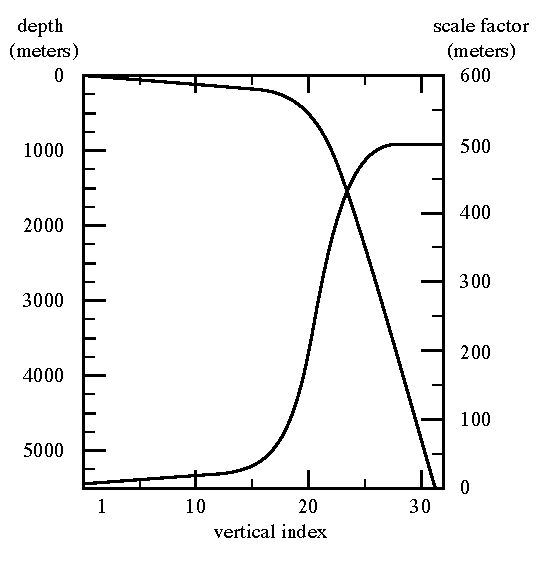
\includegraphics[width=0.90\textwidth]{./TexFiles/Figures/Fig_zgr.pdf}
\caption{ \label{Fig_zgr}    
Default vertical mesh for ORCA2: 30 ocean levels (L30). Vertical level functions for 
(a) T-point depth and (b) the associated scale factor as computed 
from \eqref{DOM_zgr_ana} using \eqref{DOM_zgr_coef} in $z$-coordinate.}
\end{center}   \end{figure}
%>>>>>>>>>>>>>>>>>>>>>>>>>>>>

The reference coordinate transformation $z_0 (k)$ defines the arrays $gdept_0$ 
and $gdepw_0$ for $t$- and $w$-points, respectively. As indicated on 
Fig.\ref{Fig_index_vert} \jp{jpk} is the number of $w$-levels. $gdepw_0(1)$ is the 
ocean surface. There are at most \jp{jpk}-1 $t$-points inside the ocean, the 
additional $t$-point at $jk=jpk$ is below the sea floor and is not used. 
The vertical location of $w$- and $t$-levels is defined from the analytic expression 
of the depth $z_0(k)$ whose analytical derivative with respect to $k$ provides the 
vertical scale factors. The user must provide the analytical expression of both 
$z_0$ and its first derivative with respect to $k$. This is done in routine \mdl{domzgr} 
through statement functions, using parameters provided in the \ngn{namcfg} namelist. 

It is possible to define a simple regular vertical grid by giving zero stretching (\np{ppacr=0}). 
In that case, the parameters \jp{jpk} (number of $w$-levels) and \np{pphmax} 
(total ocean depth in meters) fully define the grid. 

For climate-related studies it is often desirable to concentrate the vertical resolution 
near the ocean surface. The following function is proposed as a standard for a 
$z$-coordinate (with either full or partial steps): 
\begin{equation} \label{DOM_zgr_ana}
\begin{split}
 z_0 (k) 	&= h_{sur} -h_0 \;k-\;h_1 \;\log \left[ {\,\cosh \left( {{(k-h_{th} )} / {h_{cr} }} \right)\,} \right] \\ 
 e_3^0 (k) 	&= \left| -h_0 -h_1 \;\tanh \left( {{(k-h_{th} )} / {h_{cr} }} \right) \right| 
\end{split}
\end{equation}
where $k=1$ to \jp{jpk} for $w$-levels and $k=1$ to $k=1$ for $T-$levels. Such an 
expression allows us to define a nearly uniform vertical location of levels at the 
ocean top and bottom with a smooth hyperbolic tangent transition in between 
(Fig.~\ref{Fig_zgr}).

The most used vertical grid for ORCA2 has $10~m$ ($500~m)$ resolution in the 
surface (bottom) layers and a depth which varies from 0 at the sea surface to a 
minimum of $-5000~m$. This leads to the following conditions:
\begin{equation} \label{DOM_zgr_coef}
\begin{split}
 e_3 (1+1/2)		&=10. \\ 
 e_3 (jpk-1/2)	&=500. \\ 
 z(1)			&=0. \\ 
 z(jpk)			&=-5000. \\ 
\end{split}
\end{equation}

With the choice of the stretching $h_{cr} =3$ and the number of levels 
\jp{jpk}=$31$, the four coefficients $h_{sur}$, $h_{0}$, $h_{1}$, and $h_{th}$ in 
\eqref{DOM_zgr_ana} have been determined such that \eqref{DOM_zgr_coef} is 
satisfied, through an optimisation procedure using a bisection method. For the first 
standard ORCA2 vertical grid this led to the following values: $h_{sur} =4762.96$, 
$h_0 =255.58, h_1 =245.5813$, and $h_{th} =21.43336$. The resulting depths and 
scale factors as a function of the model levels are shown in Fig.~\ref{Fig_zgr} and 
given in Table \ref{Tab_orca_zgr}. Those values correspond to the parameters 
\np{ppsur}, \np{ppa0}, \np{ppa1}, \np{ppkth} in \ngn{namcfg} namelist. 

Rather than entering parameters $h_{sur}$, $h_{0}$, and $h_{1}$ directly, it is 
possible to recalculate them. In that case the user sets 
\np{ppsur}=\np{ppa0}=\np{ppa1}=999999., in \ngn{namcfg} namelist, 
and specifies instead the four following parameters:
\begin{itemize}
\item 	\np{ppacr}=$h_{cr} $: stretching factor (nondimensional). The larger 
\np{ppacr}, the smaller the stretching. Values from $3$ to $10$ are usual.
\item 	\np{ppkth}=$h_{th} $: is approximately the model level at which maximum 
stretching occurs (nondimensional, usually of order 1/2 or 2/3 of \jp{jpk})
\item 	\np{ppdzmin}: minimum thickness for the top layer (in meters)
\item 	\np{pphmax}: total depth of the ocean (meters).
\end{itemize}
As an example, for the $45$ layers used in the DRAKKAR configuration those 
parameters are: \jp{jpk}=46, \np{ppacr}=9, \np{ppkth}=23.563, \np{ppdzmin}=6m, 
\np{pphmax}=5750m.

%>>>>>>>>>>>>>>>>>>>>>>>>>>>>
\begin{table}     \begin{center} \begin{tabular}{c||r|r|r|r}
\hline
\textbf{LEVEL}& \textbf{gdept}& \textbf{gdepw}& \textbf{e3t }& \textbf{e3w  } \\ \hline
1	&	\textbf{  5.00}	&       0.00 &	\textbf{ 10.00} &	 10.00 \\	\hline
2	&	\textbf{15.00}	& 	  10.00 &	\textbf{ 10.00} &	 10.00 \\	\hline
3	&	\textbf{25.00}	&	  20.00 &	\textbf{ 10.00} & 	 10.00 \\	\hline
4	&	\textbf{35.01}	&	  30.00 & 	\textbf{ 10.01} & 	 10.00 \\	\hline
5	&	\textbf{45.01}	&	  40.01 &	\textbf{ 10.01} &	 10.01 \\	\hline
6	&	\textbf{55.03}	&	  50.02 &	\textbf{ 10.02} & 	 10.02 \\	\hline
7	&	\textbf{65.06}	&	  60.04 &	\textbf{ 10.04} &	 10.03 \\	\hline
8	&	\textbf{75.13}	&	  70.09 &	\textbf{ 10.09} &	 10.06 \\	\hline
9	&	\textbf{85.25}	&	  80.18 &	\textbf{ 10.17} &	 10.12 \\	\hline
10	& 	\textbf{95.49}	& 	  90.35 &	\textbf{ 10.33} &	 10.24 \\	\hline
11	& 	\textbf{105.97}	& 	 100.69 &	\textbf{ 10.65} &	 10.47 \\	\hline
12	& 	\textbf{116.90}	& 	 111.36 &	\textbf{ 11.27} &	 10.91 \\	\hline
13	& 	\textbf{128.70}	& 	 122.65 &	\textbf{ 12.47} &	 11.77 \\	\hline
14	& 	\textbf{142.20}	& 	 135.16 &	\textbf{ 14.78} &	 13.43 \\	\hline
15	& 	\textbf{158.96}	& 	 150.03 &	\textbf{ 19.23} &	 16.65 \\	\hline
16	& 	\textbf{181.96}	& 	 169.42 &	\textbf{ 27.66} &	 22.78 \\	\hline
17	& 	\textbf{216.65}	& 	 197.37 & 	\textbf{ 43.26} &	 34.30 \\ \hline
18	& 	\textbf{272.48}	& 	 241.13 & 	\textbf{ 70.88} &	 55.21 \\ \hline
19	& 	\textbf{364.30}	& 	 312.74 & 	\textbf{116.11} &	 90.99 \\ \hline
20	& 	\textbf{511.53}	& 	 429.72 & 	\textbf{181.55} & 	146.43 \\ \hline
21	& 	\textbf{732.20}	& 	 611.89 & 	\textbf{261.03} & 	220.35 \\ \hline
22	& 	\textbf{1033.22}&	 872.87 & 	\textbf{339.39} & 	301.42 \\ \hline
23	& 	\textbf{1405.70}&	1211.59 & \textbf{402.26} & 	373.31 \\ \hline
24	& 	\textbf{1830.89}&	1612.98 & \textbf{444.87} & 	426.00 \\ \hline
25	& 	\textbf{2289.77}&	2057.13 & \textbf{470.55} & 	459.47 \\ \hline
26	& 	\textbf{2768.24}&	2527.22 & \textbf{484.95} & 	478.83 \\ \hline
27	& 	\textbf{3257.48}&	3011.90 & \textbf{492.70} & 	489.44 \\ \hline
28	& 	\textbf{3752.44}&	3504.46 & \textbf{496.78} & 	495.07 \\ \hline
29	& 	\textbf{4250.40}&	4001.16 & \textbf{498.90} & 	498.02 \\ \hline
30	& 	\textbf{4749.91}&	4500.02 & \textbf{500.00} &	499.54 \\ \hline
31	& 	\textbf{5250.23}&	5000.00 &	\textbf{500.56} &	500.33 \\ \hline
\end{tabular} \end{center} 
\caption{ \label{Tab_orca_zgr}   
Default vertical mesh in $z$-coordinate for 30 layers ORCA2 configuration as computed 
from \eqref{DOM_zgr_ana} using the coefficients given in \eqref{DOM_zgr_coef}}
\end{table}
%>>>>>>>>>>>>>>>>>>>>>>>>>>>>

% -------------------------------------------------------------------------------------------------------------
%        z-coordinate with partial step
% -------------------------------------------------------------------------------------------------------------
\subsection   [$z$-coordinate with partial step (\np{ln\_zps})]
			{$z$-coordinate with partial step (\np{ln\_zps}=.true.)}
\label{DOM_zps}
%--------------------------------------------namdom-------------------------------------------------------
\namdisplay{namdom} 
%--------------------------------------------------------------------------------------------------------------

In $z$-coordinate partial step, the depths of the model levels are defined by the 
reference analytical function $z_0 (k)$ as described in the previous 
section, \emph{except} in the bottom layer. The thickness of the bottom layer is 
allowed to vary as a function of geographical location $(\lambda,\varphi)$ to allow a 
better representation of the bathymetry, especially in the case of small 
slopes (where the bathymetry varies by less than one level thickness from 
one grid point to the next). The reference layer thicknesses $e_{3t}^0$ have been 
defined in the absence of bathymetry. With partial steps, layers from 1 to 
\jp{jpk}-2 can have a thickness smaller than $e_{3t}(jk)$. The model deepest layer (\jp{jpk}-1) 
is allowed to have either a smaller or larger thickness than $e_{3t}(jpk)$: the 
maximum thickness allowed is $2*e_{3t}(jpk-1)$. This has to be kept in mind when 
specifying values in \ngn{namdom} namelist, as the maximum depth \np{pphmax} 
in partial steps: for example, with 
\np{pphmax}$=5750~m$ for the DRAKKAR 45 layer grid, the maximum ocean depth 
allowed is actually $6000~m$ (the default thickness $e_{3t}(jpk-1)$ being $250~m$). 
Two variables in the namdom namelist are used to define the partial step 
vertical grid. The mimimum water thickness (in meters) allowed for a cell 
partially filled with bathymetry at level jk is the minimum of \np{rn\_e3zps\_min} 
(thickness in meters, usually $20~m$) or $e_{3t}(jk)*\np{rn\_e3zps\_rat}$ (a fraction, 
usually 10\%, of the default thickness $e_{3t}(jk)$).

 \colorbox{yellow}{Add a figure here of pstep especially at last ocean level }

% -------------------------------------------------------------------------------------------------------------
%        s-coordinate
% -------------------------------------------------------------------------------------------------------------
\subsection   [$s$-coordinate (\np{ln\_sco})]
		     {$s$-coordinate (\np{ln\_sco}=true)}
\label{DOM_sco}
%------------------------------------------nam_zgr_sco---------------------------------------------------
\namdisplay{namzgr_sco} 
%--------------------------------------------------------------------------------------------------------------
Options are defined in \ngn{namzgr\_sco}.
In $s$-coordinate (\np{ln\_sco}~=~true), the depth and thickness of the model 
levels are defined from the product of a depth field and either a stretching 
function or its derivative, respectively:

\begin{equation} \label{DOM_sco_ana}
\begin{split}
 z(k) 		&= h(i,j) \; z_0(k)	\\
 e_3(k)	&= h(i,j) \; z_0'(k)
\end{split}
\end{equation}

where $h$ is the depth of the last $w$-level ($z_0(k)$) defined at the $t$-point 
location in the horizontal and $z_0(k)$ is a function which varies from $0$ at the sea 
surface to $1$ at the ocean bottom. The depth field $h$ is not necessary the ocean 
depth, since a mixed step-like and bottom-following representation of the 
topography can be used (Fig.~\ref{Fig_z_zps_s_sps}d-e) or an envelop bathymetry can be defined (Fig.~\ref{Fig_z_zps_s_sps}f).
The namelist parameter \np{rn\_rmax} determines the slope at which the terrain-following coordinate intersects the sea bed and becomes a pseudo z-coordinate. The coordinate can also be hybridised by specifying \np{rn\_sbot\_min} and \np{rn\_sbot\_max} as the minimum and maximum depths at which the terrain-following vertical coordinate is calculated.

Options for stretching the coordinate are provided as examples, but care must be taken to ensure that the vertical stretch used is appropriate for the application.

The original default NEMO s-coordinate stretching is available if neither of the other options are specified as true (\np{ln\_sco\_SH94}~=~false and \np{ln\_sco\_SF12}~=~false.) This uses a depth independent $\tanh$ function for the stretching \citep{Madec_al_JPO96}:

\begin{equation}
  z = s_{min}+C\left(s\right)\left(H-s_{min}\right)
  \label{eq:SH94_1}
\end{equation}

where $s_{min}$ is the depth at which the s-coordinate stretching starts and allows a z-coordinate to placed on top of the stretched coordinate, and z is the depth (negative down from the asea surface).

\begin{equation}
  s = -\frac{k}{n-1} \quad \text{ and } \quad 0 \leq k \leq n-1
  \label{eq:s}
\end{equation}

\begin{equation} \label{DOM_sco_function}
\begin{split}
C(s)	&=  \frac{ \left[	  \tanh{ \left( \theta \, (s+b) \right)} 
	  	 			- \tanh{ \left(  \theta \, b      \right)}  \right]}
		      {2\;\sinh \left( \theta \right)}
\end{split}
\end{equation}

A stretching function, modified from the commonly used \citet{Song_Haidvogel_JCP94} stretching (\np{ln\_sco\_SH94}~=~true), is also available and is more commonly used for shelf seas modelling:

\begin{equation}
  C\left(s\right) =   \left(1 - b \right)\frac{ \sinh\left( \theta s\right)}{\sinh\left(\theta\right)} +      \\
  b\frac{ \tanh \left[ \theta \left(s + \frac{1}{2} \right)\right] - \tanh\left(\frac{\theta}{2}\right)}{ 2\tanh\left (\frac{\theta}{2}\right)}
  \label{eq:SH94_2}
\end{equation}

%>>>>>>>>>>>>>>>>>>>>>>>>>>>>
\begin{figure}[!ht]    \begin{center}
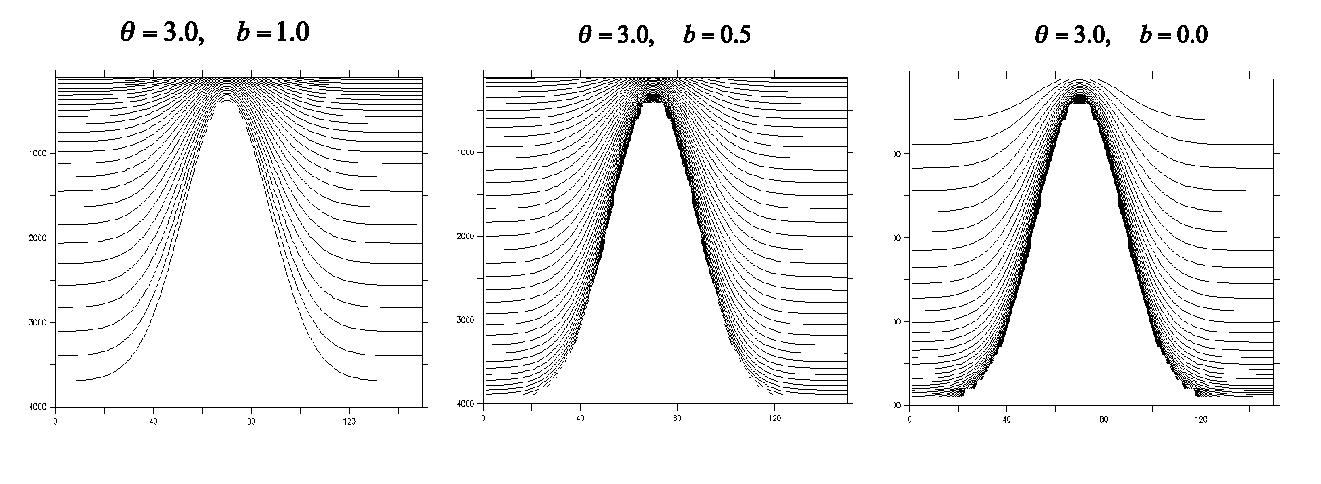
\includegraphics[width=1.0\textwidth]{./TexFiles/Figures/Fig_sco_function.pdf}
\caption{  \label{Fig_sco_function}   
Examples of the stretching function applied to a seamount; from left to right: 
surface, surface and bottom, and bottom intensified resolutions}
\end{center}   \end{figure}
%>>>>>>>>>>>>>>>>>>>>>>>>>>>>

where $H_c$ is the critical depth (\np{rn\_hc}) at which the coordinate transitions from pure $\sigma$ to the stretched coordinate,  and $\theta$ (\np{rn\_theta}) and $b$ (\np{rn\_bb}) are the surface and 
bottom control parameters such that $0\leqslant \theta \leqslant 20$, and 
$0\leqslant b\leqslant 1$. $b$ has been designed to allow surface and/or bottom 
increase of the vertical resolution (Fig.~\ref{Fig_sco_function}).

Another example has been provided at version 3.5 (\np{ln\_sco\_SF12}) that allows a fixed surface resolution in an analytical terrain-following stretching \citet{Siddorn_Furner_OM12}. In this case the a stretching function $\gamma$ is defined such that:

\begin{equation}
z = -\gamma h \quad \text{ with } \quad 0 \leq \gamma \leq 1
\label{eq:z}
\end{equation}

The function is defined with respect to $\sigma$, the unstretched terrain-following coordinate:

\begin{equation} \label{DOM_gamma_deriv}
\gamma= A\left(\sigma-\frac{1}{2}\left(\sigma^{2}+f\left(\sigma\right)\right)\right)+B\left(\sigma^{3}-f\left(\sigma\right)\right)+f\left(\sigma\right)
\end{equation}

Where:
\begin{equation} \label{DOM_gamma}
f\left(\sigma\right)=\left(\alpha+2\right)\sigma^{\alpha+1}-\left(\alpha+1\right)\sigma^{\alpha+2} \quad \text{ and } \quad \sigma = \frac{k}{n-1} 
\end{equation}

This gives an analytical stretching of $\sigma$ that is solvable in $A$ and $B$ as a function of the user prescribed stretching parameter $\alpha$ (\np{rn\_alpha}) that stretches towards the surface ($\alpha > 1.0$) or the bottom ($\alpha < 1.0$) and user prescribed surface (\np{rn\_zs}) and bottom depths. The bottom cell depth in this example is given as a function of water depth:

\begin{equation} \label{DOM_zb}
Z_b= h a + b
\end{equation}

where the namelist parameters \np{rn\_zb\_a} and \np{rn\_zb\_b} are $a$ and $b$ respectively.

%>>>>>>>>>>>>>>>>>>>>>>>>>>>>
\begin{figure}[!ht]
   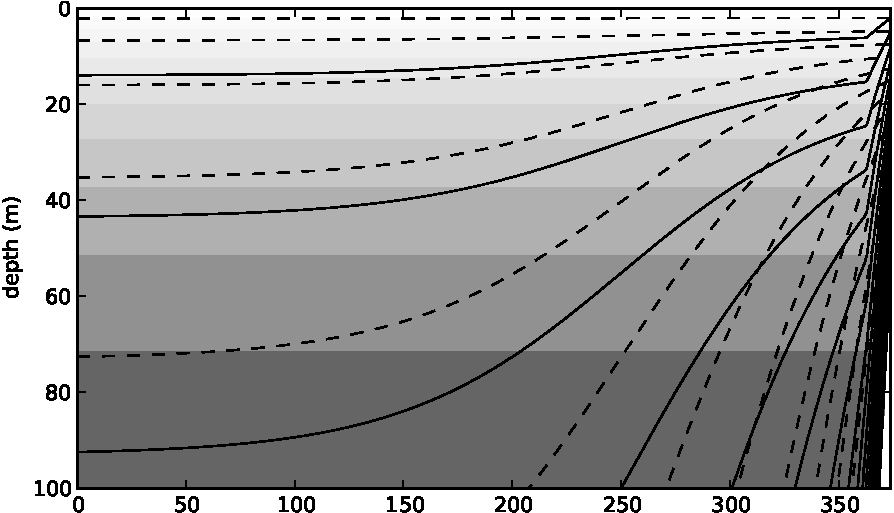
\includegraphics[width=1.0\textwidth]{./TexFiles/Figures/FIG_DOM_compare_coordinates_surface.pdf}
        \caption{A comparison of the \citet{Song_Haidvogel_JCP94} $S$-coordinate (solid lines), a 50 level $Z$-coordinate (contoured surfaces) and the \citet{Siddorn_Furner_OM12} $S$-coordinate (dashed lines) in the surface 100m for a idealised bathymetry that goes from 50m to 5500m depth. For clarity every third coordinate surface is shown.}
    \label{fig_compare_coordinates_surface}
\end{figure}
%>>>>>>>>>>>>>>>>>>>>>>>>>>>>

This gives a smooth analytical stretching in computational space that is constrained to given specified surface and bottom grid cell thicknesses in real space. This is not to be confused with the hybrid schemes that superimpose geopotential coordinates on terrain following coordinates thus creating a non-analytical vertical coordinate that therefore may suffer from large gradients in the vertical resolutions. This stretching is less straightforward to implement than the \citet{Song_Haidvogel_JCP94} stretching, but has the advantage of resolving diurnal processes in deep water and has generally flatter slopes.

As with the \citet{Song_Haidvogel_JCP94} stretching the stretch is only applied at depths greater than the critical depth $h_c$. In this example two options are available in depths shallower than $h_c$, with pure sigma being applied if the \np{ln\_sigcrit} is true and pure z-coordinates if it is false (the z-coordinate being equal to the depths of the stretched coordinate at $h_c$.

Minimising the horizontal slope of the vertical coordinate is important in terrain-following systems as large slopes lead to hydrostatic consistency. A hydrostatic consistency parameter diagnostic following \citet{Haney1991} has been implemented, and is output as part of the model mesh file at the start of the run.

% -------------------------------------------------------------------------------------------------------------
%        z*- or s*-coordinate
% -------------------------------------------------------------------------------------------------------------
\subsection{$z^*$- or $s^*$-coordinate (add \key{vvl}) }
\label{DOM_zgr_vvl}

This option is described in the Report by Levier \textit{et al.} (2007), available on 
the \NEMO web site. 

%gm% key advantage: minimise the diffusion/dispertion associated with advection in response to high frequency surface disturbances

% -------------------------------------------------------------------------------------------------------------
%        level bathymetry and mask 
% -------------------------------------------------------------------------------------------------------------
\subsection{level bathymetry and mask}
\label{DOM_msk}

Whatever the vertical coordinate used, the model offers the possibility of 
representing the bottom topography with steps that follow the face of the 
model cells (step like topography) \citep{Madec_al_JPO96}. The distribution of 
the steps in the horizontal is defined in a 2D integer array, mbathy, which 
gives the number of ocean levels ($i.e.$ those that are not masked) at each 
$t$-point. mbathy is computed from the meter bathymetry using the definiton of 
gdept as the number of $t$-points which gdept $\leq$ bathy. 

Modifications of the model bathymetry are performed in the \textit{bat\_ctl} 
routine (see \mdl{domzgr} module) after mbathy is computed. Isolated grid points 
that do not communicate with another ocean point at the same level are eliminated.

From the \textit{mbathy} array, the mask fields are defined as follows:
\begin{align*}
tmask(i,j,k) &= \begin{cases}   \; 1&   \text{ if $k\leq mbathy(i,j)$  }    \\
                                                \; 0&   \text{ if $k\leq mbathy(i,j)$  }    \end{cases}     \\
umask(i,j,k) &=         \; tmask(i,j,k) \ * \ tmask(i+1,j,k)	\\
vmask(i,j,k) &=         \; tmask(i,j,k) \ * \ tmask(i,j+1,k)	\\
fmask(i,j,k) &=         \; tmask(i,j,k) \ * \ tmask(i+1,j,k)	\\
                   & \ \ \, * tmask(i,j,k) \ * \ tmask(i+1,j,k)
\end{align*}

Note that \textit{wmask} is not defined as it is exactly equal to \textit{tmask} with 
the numerical indexing used (\S~\ref{DOM_Num_Index}). Moreover, the 
specification of closed lateral boundaries requires that at least the first and last 
rows and columns of the \textit{mbathy} array are set to zero. In the particular 
case of an east-west cyclical boundary condition, \textit{mbathy} has its last 
column equal to the second one and its first column equal to the last but one 
(and so too the mask arrays) (see \S~\ref{LBC_jperio}).

%%%
\gmcomment{   \colorbox{yellow}{Add one word on tricky trick !} mbathy in further modified in zdfbfr{\ldots}.  }
%%%

% ================================================================
% Domain: Initial State (dtatsd & istate)
% ================================================================
\section  [Domain: Initial State (\textit{istate and dtatsd})]
		{Domain: Initial State \small{(\mdl{istate} and \mdl{dtatsd} modules)} }
\label{DTA_tsd}
%-----------------------------------------namtsd-------------------------------------------
\namdisplay{namtsd} 
%------------------------------------------------------------------------------------------

Options are defined in \ngn{namtsd}.
By default, the ocean start from rest (the velocity field is set to zero) and the initialization of 
temperature and salinity fields is controlled through the \np{ln\_tsd\_ini} namelist parameter.
\begin{description}
\item[ln\_tsd\_init = .true.]  use a T and S input files that can be given on the model grid itself or 
on their native input data grid. In the latter case, the data will be interpolated on-the-fly both in the 
horizontal and the vertical to the model grid (see \S~\ref{SBC_iof}). The information relative to the 
input files are given in the \np{sn\_tem} and \np{sn\_sal} structures. 
The computation is done in the \mdl{dtatsd} module.
\item[ln\_tsd\_init = .false.] use constant salinity value of 35.5 psu and an analytical profile of temperature
(typical of the tropical ocean), see \rou{istate\_t\_s} subroutine called from \mdl{istate} module.
\end{description}
